
\section{QUY TẮC ĐẾM}

\subsection{LÝ THUYẾT CẦN NHỚ}
\subsubsection{Quy tắc cộng và sơ đồ hình cây}
\begin{itemize}
	\item [\iconMT] \indam{ Quy tắc cộng:} 
	\begin{tcolorbox}[colframe=orange,colback=orange!3,boxrule=0.2mm]
		Giả sử một công việc được hoàn thành bởi một trong \textbf{hai} phương án khác nhau: 
		\begin{itemize}
			\item [$\bullet$] Phương án 1 có $n_1$ cách thực hiện; 
			\item [$\bullet$] Phương án 2 có $n_2$ cách thực hiện không trùng với bất kỳ cách nào của hành động thứ nhất.
		\end{itemize}
		Khi đó, số cách thực hiện công việc là $n_1+n_2$ cách.
	\end{tcolorbox}
	\item [\iconMT] \indam{Sơ đồ hình cây:}
		\immini{
				Là sơ đồ bắt đầu tại một nút duy nhất với các nhánh tỏa ra các nút bổ sung.
				Trong các bài toán đếm, ta thường dùng sơ đồ hình cây để minh họa, giúp cho việc đếm thuận tiện và không bỏ sót trường hợp.
	 }
		{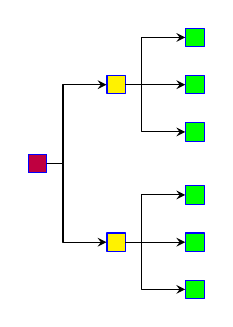
\begin{tikzpicture}[font=\footnotesize, line join=round, line cap=round, >=stealth,scale=2]
				\path(0,0)node(a)[draw=blue,fill=purple]{}
				++(0.5,0.5)node[draw=blue,fill=yellow](b){}
				(a)++(0.5,-0.5)node[draw=blue,fill=yellow](c){}
				;
				\path
				(b)++(0.5,0.3)node(b1)[draw=blue,fill=green]{ }
				(b)++(0.5,0)node(b2)[draw=blue,fill=green]{ }
				(b)++(0.5,-0.3)node(b3)[draw=blue,fill=green]{}
				;
				\path
				(c)++(0.5,0.3)node(c1)[draw=blue,fill=green]{ }
				(c)++(0.5,0)node(c2)[draw=blue,fill=green]{ } 
				(c)++(0.5,-0.3)node(c3)[draw=blue,fill=green]{ }
				;
				\draw[-stealth,outer sep=0,inner sep=0](a.east)--++(0.1,0)|-(b.west);
				\draw[-stealth,outer sep=0,inner sep=0](a.east)--++(0.1,0)|-(c.west);
				\draw[-stealth,outer sep=0,inner sep=0](b.east)--++(0.1,0)|-(b1.west);
				\draw[-stealth,outer sep=0,inner sep=0](b.east)--++(0.1,0)|-(b2.west);
				\draw[-stealth,outer sep=0,inner sep=0](b.east)--++(0.1,0)|-(b3.west);
				\draw[-stealth,outer sep=0,inner sep=0](c.east)--++(0.1,0)|-(c1.west);
				\draw[-stealth,outer sep=0,inner sep=0](c.east)--++(0.1,0)|-(c2.west);
				\draw[-stealth,outer sep=0,inner sep=0](c.east)--++(0.1,0)|-(c3.west);
		\end{tikzpicture}}
\end{itemize}

\subsubsection{Quy tắc nhân}
\begin{itemize}
	\item [\iconMT] \indam{Quy tắc nhân:} 
	\begin{tcolorbox}[colframe=orange,colback=orange!3,boxrule=0.2mm]
		Giải sử một công việc được hoàn thành bởi \textbf{hai} công đoạn \textbf{liên tiếp} nhau:
		\begin{itemize}
			\item [$\bullet$] Công đoạn 1 có $m_1$ cách thực hiện, 
			\item [$\bullet$] Với mỗi cách thực hiện công đoạn 1, có  $m_2$ cách thực hiện công đoạn 2.
		\end{itemize}
		Khi đó, số cách thực hiện công việc là $m_1 \cdot m_2$ cách.
	\end{tcolorbox}
	\item [\iconMT] \indam{Lưu ý:} Quy tắc nhân áp dụng để tính số cách thực hiên công việc có nhiều công đoạn, các công đoạn nối tiếp nhau và những công đoạn này độc lập nhau.
\end{itemize}

\subsection{RÈN LUYỆN KĨ NĂNG GIẢI TOÁN}
\begin{dang}{Quy tắc cộng và sơ đồ hình cây}
\end{dang}

\begin{vd}%[Tex hóa SGK CD-CT,T7/22, TVN-001]%[1D2Y1-1]
	Bạn Hương có $ 3 $ chiếc quần khác màu lần lượt là xám, đen, nâu nhạt và $ 4 $ chiếc áo sơ mi cũng khác màu lần lượt là hồng, vàng, xanh, tím. Tìm số cách ban Hương có thể chọn ra
	\begin{enumEX}{3}
		\item $ 1 $ chiếc quần;
		\item $ 1 $ chiếc áo sơ mi;
		\item $ 1 $ bộ quần áo.
	\end{enumEX}
	\loigiai{
	}
\end{vd} \dongcham{6}

\begin{vd}
	Một bộ sưu tập gồm $15$ viên bi pha lê và $12$ viên bi thủy tinh, tất cả đều có hoa văn khác nhau. Hỏi người sưu tầm có bao nhiêu cách để mang đúng $1$ viên bi đi tham dự triển lãm?
	\loigiai{
		Để chọn $1$ viên bi đi triển lãm, người sưu tầm có thể chọn bi pha lê hoặc bi thủy tinh:
		\begin{itemize}
			\item Nếu chọn bi pha lê: có $15$ cách.
			\item Nếu chọn bi thủy tinh: có $12$ cách.
		\end{itemize}
		Theo quy tắc cộng, số cách chọn $1$ viên bi là: $15 + 12 = 27$ (cách).
	}
\end{vd}\dongcham{5}

\begin{vd}%[1D2B1-1]%Ví dụ 3.
	Trên bàn có $8$ cây bút chì khác nhau, $6$ cây bút bi khác nhau và $10$ cuốn tập khác nhau. Một học sinh muốn chọn một đồ vật duy nhất hoặc một cây bút chì hoặc một cây bút bi hoặc một cuốn tập thì số cách chọn khác nhau bằng bao nhiêu?
	\loigiai{
		\begin{itemize}
			\item Nếu chọn một cây bút chì thì sẽ có $8$ cách.
			\item Nếu chọn một cây bút bi thì sẽ có $6$ cách.
			\item Nếu chọn một cuốn tập thì sẽ có $10$ cách.
		\end{itemize}
		Theo qui tắc cộng, ta có $8+6+10=24$ cách.}
\end{vd} \dongcham{5}

\begin{dang}{Quy tắc nhân}
\end{dang}

\begin{vd}
	Một giáo viên cần chọn ra một bạn nam và một bạn nữ để làm MC cho chương trình văn nghệ của trường. Biết rằng trong câu lạc bộ MC có $8$ bạn nam và $10$ bạn nữ có năng lực phù hợp. Hỏi giáo viên đó có bao nhiêu cách phân công?
	\loigiai{
		Việc phân công MC gồm $2$ bước:
		\begin{itemize}
			\item Bước 1: Chọn $1$ bạn nam từ $8$ bạn nam, có $8$ cách.
			\item Bước 2: Chọn $1$ bạn nữ từ $10$ bạn nữ, có $10$ cách.
		\end{itemize}
		Theo quy tắc nhân, tổng số cách chọn $2$ bạn làm MC là: $8 \times 10 = 80$ (cách).
	}
\end{vd}
\dongcham{4}
\begin{vd}
	Trên kệ sách có 5 sách Toán, 6 sách Lý và 7 sách Văn học. Có bao nhiêu cách chọn ra 3 quyển sách sao cho 3 quyển được chọn có đủ cả ba loại.
	\loigiai{
	}
\end{vd} \dongcham{4}


\begin{vd}
	Một người muốn tự lắp ráp một bộ máy tính để bàn. Cửa hàng linh kiện hiện có $5$ loại CPU, $4$ loại bo mạch chủ (Mainboard), $3$ loại RAM và $6$ loại vỏ máy (Case). Biết rằng tất cả các linh kiện này đều tương thích với nhau. Hỏi người đó có bao nhiêu cách chọn cấu hình máy tính gồm $1$ CPU, $1$ Mainboard, $1$ RAM và $1$ vỏ máy?
	\loigiai{
		Việc chọn cấu hình máy tính là việc chọn lần lượt các linh kiện, gồm $4$ công đoạn:
		\begin{itemize}
			\item Chọn CPU: có $5$ cách.
			\item Chọn Mainboard: có $4$ cách.
			\item Chọn RAM: có $3$ cách.
			\item Chọn vỏ máy (Case): có $6$ cách.
		\end{itemize}
		Vì các linh kiện đều tương thích nên các lựa chọn hoàn toàn độc lập với nhau. Áp dụng quy tắc nhân, số cách chọn cấu hình máy tính là: $5 \times 4 \times 3 \times 6 = 360$ (cách).
	}
\end{vd}
\dongcham{4}

\begin{vd}%[1D2B1-2]
	\immini{Tung một con xúc xắc ba lần liên tiếp và ghi lại kết quả (chẳng hạn, $1-2-4$ nếu số chấm xuất hiện lần lượt là $ 1 $, $ 4 $ và $ 2 $). Có tất cả bao nhiêu kết quả khác nhau có thể xảy ra? 
	}{
		\begin{tikzpicture}
			\tikzset{motcham/.pic={
					\begin{scope}[rounded corners=2mm]
						\def\a{2}
						\path(0,0)coordinate(A)++(-30:0.85*\a)coordinate(B)(1.5*\a,0)coordinate(C)($(A)+(C)-(B)$)coordinate(D);
						\path[shift={(0,\a)}](0,0)coordinate(A')++(-30:0.85*\a)coordinate(B')(1.5*\a,0)coordinate(C')($(A')+(C')-(B')$)coordinate(D');
						\fill[gray,draw=gray](A)--(A')--(D')--(C')--(C)--(B)--cycle;
						\draw[fill=gray!30,draw=gray](B)--(C)--(C')--(B')--cycle (A')--(B')--(C')--(D')--cycle (A)--(A')--(B')--(B)--cycle;
						\fill[ball color=red,yscale=0.5,draw=red!30]($(A')!0.5!(C')$)circle(0.25*\a)($(A')!0.5!(C')$)circle(0.25*\a);
						\path($(A')!0.5!(B')$)coordinate(M')($(A)!0.5!(B)$)coordinate(M);
						\fill[ball color=red,yslant=-0.3,,draw=red!30]($(M)!1/3!(M')$)circle(0.125*\a)($(M)!2/3!(M')$)circle(0.125*\a);
						\path($(B')!1/3!(C')$)coordinate(N')($(B) !1/3!(C)$)coordinate(N)($(B')!2/3!(C')$)coordinate(P')($(B)!2/3!(C)$)coordinate(P);
						\fill[ball color=red,yslant=0.3,draw=red!30]($(N)!1/3!(N')$)circle(0.1*\a)($(N)!2/3!(N')$)circle(0.1*\a)($(P)!1/3!(P')$)circle(0.1*\a)($(P)!2/3!(P')$)circle(0.1*\a);
					\end{scope}
			}}
			\path(0,0)pic{motcham};
	\end{tikzpicture}}
	\loigiai{
		Có thể coi việc tung con xúc xắc ba lần liên tiếp là công việc gồm ba công đoạn, mỗi công đoạn là một lần tung. Mỗi lần tung đều có 6 khả năng khác nhau xảy ra (số chấm xuất hiện là $1;2;\ldots;6$). Do đó, theo quy tắc nhân, ta có $6 \cdot 6 \cdot 6=216$ kết quả khác nhau có thể xảy ra.}
\end{vd} \dongcham{3}

\begin{vd}%[1D2B1-2]
	Tung một đồng xu $ 5 $ lần liên tiếp và ghi lại kết quả (ví dụ dùng kí hiệu $ SSNSN $ để chỉ kết quả $ 5 $ lần tung lần lượt là sấp, sấp, ngửa, sấp, ngửa). Có bao nhiêu kết quả khác nhau có thể xảy ra?
	\loigiai{
		Có thể coi việc tung đồng xu $ 5 $ lần liên tiếp là công việc gồm $ 5 $ công đoạn. Mỗi công đoạn có $ 2 $ phương án thực hiện, tương ứng đồng xu xuất hiện sấp hay ngửa. Do đó, theo quy tắc nhân, có $2 \cdot 2 \cdot 2 \cdot 2 \cdot 2=32$ kết quả có thể của việc tung đồng xu $ 5 $ lần liên tiếp.}
\end{vd} \dongcham{4}


\begin{vd}
	Biển đăng ký xe ô tô có hai chữ cái đứng đầu (trong bảng $26$ chữ cái, không dùng các chữ I và O) và tiếp theo 7 chữ số. Chữ số đầu tiên khác $0$. Hỏi số ô tô được đăng ký biển xe như thế nhiều nhất có thể là bao nhiêu?
	\hspace*{2cm} {\sf\fontsize{10pt}{1pt}\selectfont Đáp số: $5184.10^6$}
	\loigiai{
		Do không dùng các chữ I và O nên mỗi chữ cái trong biển đăng ký xe ô tô đều có 24 cách chọn.\\
		Do chữ số đầu tiên khác $0$ nên có 9 cách chọn chữ số đầu tiên, mỗi chữ số còn lại đều có 10 cách chọn.\\
		Vậy số ô tô được đăng ký biển xe như thế nhiều nhất có thể là $24.24.9.10^6=5184.10^6$
	}
\end{vd} \dongcham{6}

\begin{dang}{Kết hợp quy tắc cộng và quy tắc nhân}
\end{dang}

\begin{vd}
	Một người có 7 cái áo trong đó có 3 áo trắng và 5 cái cà vạt trong đó có hai cà vạt màu vàng. Hỏi người đó có bao nhiêu cách chọn áo - cà vạt nếu
	\begin{tasks}(1)
		\task Chọn áo nào cũng được và cà vạt nào cũng được?
		\task Chọn áo trắng thì không chọn cà vạt màu vàng?
	\end{tasks}
\end{vd} \dongcham{8}

\begin{vd}%[1D2K1-3]%
	Một hộp chứa $10$ quả cầu màu đỏ được đánh số từ $1$ đến $10$ và $15$ quả cầu màu xanh được đánh số từ $1$ đến $15$. Chọn ngẫu nhiên $2$ quả cầu. Hỏi có bao nhiêu cách để chọn được hai quả cầu khác màu và tổng của các số trên hai quả cầu là một số lẻ?
	\loigiai{
		Để tổng của hai số là một số lẻ thì một số là số lẻ và số còn lại là số chẵn. Mặt khác, do hai quả cầu được chọn khác nhau nên ta sẽ chọn theo cách sau đây:\\
		\textbf{Trường hợp 1:} Chọn quả đỏ số chẵn và quả xanh số lẻ.\\
		Bước 1: Chọn $1$ quả cầu đỏ, có $5$ cách.\\
		Bước 2: Chọn $1$ quả cầu xanh, có $8$ cách.\\
		Suy ra có $5.8=40$ cách.\\
		\textbf{Trường hợp 2:} Chọn quả đỏ số lẻ và quả xanh số chẵn.\\
		Bước 1: Chọn $1$ quả cầu đỏ, có $5$ cách.\\
		Bước 2: Chọn $1$ quả cầu xanh, có $7$ cách.\\
		Suy ra có $5.7=35$ cách.\\
		Vậy tổng cộng có tất cả $40+35=75$ cách.
	}
\end{vd} \dongcham{8}

\begin{vd}
	Hằng ngày giữa TP HCM và Hà Nội có $4$ chuyến máy bay, $6$ chuyến xe lửa và $10$ chuyến xe khách.
	\begin{enumerate}
		\item[a)] Một người muốn đi từ TP HCM ra Hà Nội thì có mấy cách lựa chọn phương tiện?
		\item[b)] Một người muốn đi du lịch từ TP HCM ra Hà Nội thì có mấy cách lựa chọn để khi đi và về bằng hai phương tiện khác nhau.
	\end{enumerate}
	\loigiai{
		\begin{enumerate}
			\item[a)] Để đi từ TP HCM ra Hà Nội (1 chiều), người đó có các phương án sau:
			\begin{itemize}
				\item Phương án 1: Đi bằng máy bay, có $4$ cách chọn chuyến.
				\item Phương án 2: Đi bằng xe lửa, có $6$ cách chọn chuyến.
				\item Phương án 3: Đi bằng xe khách, có $10$ cách chọn chuyến.
			\end{itemize}
			Theo quy tắc cộng, người đó có tổng số cách lựa chọn phương tiện là:
			$$4 + 6 + 10 = 20 \text{ (cách).}$$
			
			\item[b)] Chuyến đi du lịch bao gồm hai công đoạn: chiều đi và chiều về. Theo đề bài, phương tiện đi và về thuộc hai loại khác nhau (ví dụ: đi máy bay thì về phải bằng xe lửa hoặc xe khách). Ta chia thành 3 trường hợp:
			\begin{itemize}
				\item \textbf{Trường hợp 1:} Chiều đi bằng máy bay, chiều về bằng phương tiện khác (xe lửa hoặc xe khách). \\
				Số cách chọn chuyến đi (máy bay) là $4$ cách. \\
				Số cách chọn chuyến về (xe lửa hoặc xe khách) là $6 + 10 = 16$ cách. \\
				Theo quy tắc nhân, có $4 \cdot 16 = 64$ cách.
				
				\item \textbf{Trường hợp 2:} Chiều đi bằng xe lửa, chiều về bằng phương tiện khác (máy bay hoặc xe khách). \\
				Số cách chọn chuyến đi (xe lửa) là $6$ cách. \\
				Số cách chọn chuyến về (máy bay hoặc xe khách) là $4 + 10 = 14$ cách. \\
				Theo quy tắc nhân, có $6 \cdot 14 = 84$ cách.
				
				\item \textbf{Trường hợp 3:} Chiều đi bằng xe khách, chiều về bằng phương tiện khác (máy bay hoặc xe lửa). \\
				Số cách chọn chuyến đi (xe khách) là $10$ cách. \\
				Số cách chọn chuyến về (máy bay hoặc xe lửa) là $4 + 6 = 10$ cách. \\
				Theo quy tắc nhân, có $10 \cdot 10 = 100$ cách.
			\end{itemize}
			Theo quy tắc cộng, tổng số cách lựa chọn cho chuyến du lịch khứ hồi là:
			$$64 + 84 + 100 = 248 \text{ (cách).}$$
		\end{enumerate}
	}
\end{vd}
\dongcham{8}

\begin{dang}{Bài toán đếm số tự nhiên}
	Giả sử số tự nhiên cần lập có 3 chữ số.
	\begin{enumerate}[1.]
		\item Bước 1: Gọi số cần lập là $\overline{abc}$, với $a \ne 0$.
		\item Bước 2: Từ dữ kiện bài toán, ta tính toán số cách chọn cho từng vị trí $a$, $b$, $c$. 
		\begin{itemize}
			\item Chọn $a$ có $m_1$ cách;
			\item Ứng với cách chọn $a$, chọn $b$ có $m_2$ cách;
			\item Ứng với cách chọn $a$ và $b$, chọn $c$ có $m_3$ cách;
		\end{itemize}
	\item Bước 3: Kết luận có $m_1 \cdot m_2 \cdot m_3$ số tự nhiên được tạo thành.
	\end{enumerate}
\end{dang}

	\begin{vd}
	Từ các chữ số $1, 2, 3, 4, 5$ có thể lập được bao nhiêu số tự nhiên gồm $3$ chữ số?
	\loigiai{
		Gọi số tự nhiên cần tìm có dạng $\overline{abc}$, trong đó $a, b, c \in \{1, 2, 3, 4, 5\}$.
		\begin{itemize}
			\item Chữ số $a$ có $5$ cách chọn.
			\item Chữ số $b$ có $5$ cách chọn.
			\item Chữ số $c$ có $5$ cách chọn.
		\end{itemize}
		Theo quy tắc nhân, số các số tự nhiên có thể lập được là: $5 \times 5 \times 5 = 125$ (số).
	}
\end{vd}
\dongcham{3}
\begin{vd}
	Từ các chữ số $1, 2, 3, 4, 5, 6$ có thể lập được bao nhiêu số tự nhiên gồm $4$ chữ số đôi một khác nhau?
	\loigiai{
		Mỗi số tự nhiên gồm $4$ chữ số đôi một khác nhau được lập từ $6$ chữ số đã cho là một chỉnh hợp chập $4$ của $6$ phần tử.
		Số lượng số tự nhiên thỏa mãn yêu cầu bài toán là:
		$$A_6^4 = \frac{6!}{(6-4)!} = 6 \times 5 \times 4 \times 3 = 360 \text{ (số)}.$$
	}
\end{vd}
\dongcham{3}
\begin{vd}
	Từ các chữ số $0, 1, 2, 3, 4, 5, 6$ có thể lập được bao nhiêu số tự nhiên gồm $3$ chữ số đôi một khác nhau?
	\loigiai{
		Gọi số tự nhiên cần tìm có dạng $\overline{abc}$, trong đó $a \neq 0$ và $a, b, c$ phân biệt thuộc tập hợp $A = \{0, 1, 2, 3, 4, 5, 6\}$.
		\begin{itemize}
			\item Chọn chữ số $a \neq 0$: có $6$ cách chọn ($a \in \{1, 2, 3, 4, 5, 6\}$).
			\item Chọn $2$ chữ số còn lại cho $b$ và $c$ từ $6$ chữ số còn lại của tập $A$ (đã bỏ đi chữ số $a$): có $A_6^2 = 30$ cách.
		\end{itemize}
		Theo quy tắc nhân, có $6 \times 30 = 180$ (số).
	}
\end{vd}
\dongcham{5}
\begin{vd}
	Từ các chữ số $1, 2, 3, 4, 5, 6, 7$ lập được bao nhiêu số tự nhiên lẻ gồm $3$ chữ số đôi một khác nhau?
	\loigiai{
		Gọi số tự nhiên cần tìm có dạng $\overline{abc}$, vì là số lẻ nên $c \in \{1, 3, 5, 7\}$.
		\begin{itemize}
			\item Chọn chữ số $c$: có $4$ cách chọn.
			\item Chọn chữ số $a$: có $6$ cách chọn (khác $c$).
			\item Chọn chữ số $b$: có $5$ cách chọn (khác $a$ và $c$).
		\end{itemize}
		Theo quy tắc nhân, số các số lập được là: $4 \times 6 \times 5 = 120$ (số).
	}
\end{vd}
\dongcham{4}
\begin{vd}
	Từ các chữ số $0, 1, 2, 3, 4, 5$ lập được bao nhiêu số tự nhiên chẵn gồm $3$ chữ số đôi một khác nhau?
	\loigiai{
		Gọi số tự nhiên cần tìm có dạng $\overline{abc}$, với $a \neq 0$. Vì số chẵn nên $c \in \{0, 2, 4\}$. Ta xét hai trường hợp:
		\begin{itemize}
			\item \textbf{Trường hợp 1:} $c = 0$.
			Chữ số $c$ có $1$ cách chọn. Hai chữ số $a, b$ được chọn từ $5$ chữ số còn lại, có $A_5^2 = 20$ cách.
			Vậy TH1 có $1 \times 20 = 20$ (số).
			\item \textbf{Trường hợp 2:} $c \in \{2, 4\}$.
			Chữ số $c$ có $2$ cách chọn.
			Chữ số $a \neq 0$ và $a \neq c$ nên $a$ có $4$ cách chọn.
			Chữ số $b \neq a$ và $b \neq c$ nên $b$ có $4$ cách chọn.
			Vậy TH2 có $2 \times 4 \times 4 = 32$ (số).
		\end{itemize}
		Theo quy tắc cộng, tổng số các số chẵn lập được là: $20 + 32 = 52$ (số).
	}
\end{vd}
\dongcham{4}
\begin{vd}
	Cho tập hợp $A= \{0;1;2;3;4;5;6;7 \}$. Hỏi từ tập $A$ có thể lập được bao nhiêu số tự nhiên gồm $5$ chữ số đôi một khác nhau sao cho một trong $3$ chữ số đầu tiên phải bằng $1$.\\
	\hspace*{6cm} {\sf\fontsize{10pt}{1pt}\selectfont Đáp số: 2280. }
	\loigiai{
		Gọi số cần tìm có dạng $\overline{abcde}$\\
		TH1: $a=1$
		\begin{itemize}
			\item $b$ có $7$ cách chọn.
			\item $c$ có $6$ cách chọn.
			\item $d$ có $5$ cách chọn.
			\item $e$ có $4$ cách chọn.
		\end{itemize}
		Nên có $7 \cdot 6 \cdot 5 \cdot 4 = 840$ số.\\
		TH2: $b=1$
		\begin{itemize}
			\item $a \neq b$, $a \neq 0$ nên $a$ có $6$ cách chọn
			\item $c$ có $6$ cách chọn.
			\item $d$ có $5$ cách chọn.
			\item $e$ có $4$ cách chọn.
		\end{itemize}
		Nên có $6 \cdot 6 \cdot 5 \cdot 4 = 720$ số.\\
		TH3: $c=1$
		\begin{itemize}
			\item $a \neq c$, $a \neq 0$ nên $a$ có $6$ cách chọn
			\item $b$ có $6$ cách chọn.
			\item $d$ có $5$ cách chọn.
			\item $e$ có $4$ cách chọn.
		\end{itemize}
		Nên có $6 \cdot 6 \cdot 5 \cdot 4 = 720$ số.\\
		Vậy có tất cả $840 + 720 + 720 = 2280$ số.
	}
\end{vd} \dongcham{14}

\begin{vd}
	Cho tập hợp $A=\{0;1;2;3;4;5\}$. Có thể lập được bao nhiêu số tự nhiên có $3$ chữ số khác nhau và lớn hơn $350$?\\
	\hspace*{6cm} {\sf\fontsize{10pt}{1pt}\selectfont Đáp số: 43 }
	\loigiai{
		Gọi số tự nhiên thỏa mãn là $\overline{abc}$. Do $\overline{abc}>350$ nên $a\in\{3;4;5\}$.
		\begin{itemize}
			\item Trường hợp $a\in\{4;5\}$: Chọn $a$ có $2$ cách, chọn $b$ có $5$ cách, chọn $c$ có $4$ cách. Vậy trường hợp này có $2\cdot 5\cdot 4=40$ số thỏa mãn.
			\item Trường hợp $a=3$, chọn $b$ có $1$ cách là $b=5$, chọn $c$ có $3$ cách (vì $c$ cần khác cả $0$). Vậy trường hợp này có $3$ số thỏa mãn.
			\item Vậy có tất cả $40+3=43$ số thỏa mãn.
		\end{itemize}
	}
\end{vd} \dongcham{14}

\subsection{BÀI TẬP TỰ LUYỆN}

\begin{baitap}
	Trong tủ quần áo của bạn An có $4$ chiếc áo khác nhau và $3$ chiếc quần khác nhau. Hỏi bạn An có bao nhiêu cách chọn $1$ bộ quần áo để mặc? \\
	\hspace*{6cm} {\sf\fontsize{10pt}{1pt}\selectfont Đáp số: 12.}
	\loigiai{
		Số cách chọn $1$ bộ quần áo là $3\cdot 4 = 12$.
	}
\end{baitap} \cham{7}



\begin{baitap}
	Một người vào cửa hàng ăn, người đó chọn thực đơn gồm $1$ món ăn trong $7$ món, $1$ loại quả tráng miệng trong $4$ loại quả tráng miệng và một nước uống trong $5$ loại nước uống. Có bao nhiêu cách chọn thực đơn.\\
	\hspace*{6cm} {\sf\fontsize{10pt}{1pt}\selectfont Đáp số: 140.}
	\loigiai{
		Việc chọn một thực đơn bao gồm $3$ công việc liên tiếp nhau
		\begin{itemize}
			\item[$\bullet$] Công việc $1$: chọn $1$ món ăn, có $7$ cách chọn.
			\item[$\bullet$] Công việc $2$: chọn $1$ loại quả tráng miệng, có $4$ cách chọn.
			\item[$\bullet$] Công việc $3$: chọn $1$ loại nước uống, có $5$ cách chọn.
		\end{itemize}
		Theo quy tắc nhân, số cách chọn một thực đơn là $7 \cdot 4 \cdot 5 = 140$ (cách).
	}
\end{baitap} \cham{7}

\begin{baitap}
	Một hộp chứa các viên bi khác nhau gồm $6$ viên bi đỏ, $9$ viên bi xanh và $5$ bi vàng. Hỏi có bao nhiêu cách chọn ra $3$ viên bi có đủ cả ba màu?\\
	\hspace*{6cm} {\sf\fontsize{10pt}{1pt}\selectfont Đáp số: 270 }
	\loigiai{
		Chọn một bi đỏ: có $6$ cách.\\
		Chọn một bi xanh: có $9$ cách.\\
		Chọn một bi vàng: có $5$ cách.\\
		Do đó có $6\times9\times5=270$ cách.}
\end{baitap} \cham{8}

\begin{baitap}%[1D2B1-1]%
	Một hội nghị $3$ nước Đông Dương có số đại biểu gồm: $10$ đại biểu Việt Nam; $8$ đại biểu Campuchia và $6$ đại biểu Lào.
	\begin{enumerate}
		\item Có bao nhiêu cách chọn một vị đại biểu để đọc diễn văn khai mạc?
		\item Có bao nhiêu cách chọn $3$ vị đại biểu của $3$ nước khác nhau làm thư ký đoàn?
		\item Có bao nhiêu cách chọn $2$ vị đại biểu của $2$ nước khác nhau để họp báo?
	\end{enumerate}
	\loigiai{
		\begin{enumerate}
			\item Có $10+8+6=24$ cách chọn $1$ vị đại biểu để đọc diễn văn khai mạc.
			\item Có $10 \cdot 8 \cdot 6=480$ cách chọn $3$ vị đại biểu của $3$ nước khác nhau làm thư kí đoàn.
			\item Để chọn $2$ vị đại biểu của $2$ nước khác nhau để họp báo ta chia thành các trường hợp sau:
			\begin{itemize}
				\item Trường hợp 1: 1 đại biểu Lào, 1 đại biểu Việt Nam có $6 \cdot 10=60$ cách.
				\item Trường hợp 2: 1 đại biểu Lào, 1 đại biểu Campuchia có $6 \cdot 8=48$ cách.
				\item Trường hợp 3: 1 đại biểu Việt Nam, 1 đại biểu Campuchia có $10 \cdot 8=80$ cách.
			\end{itemize}
			Vậy theo quy tắc cộng ta có $188$ cách để chọn $2$ đại biểu của hai nước khác nhau để họp báo.
		\end{enumerate}
	}
\end{baitap} \cham{10}

\begin{baitap}%[1D2B1-1]%[1D2B1-2]%[1D2B1-3]
	Trên giá sách có $  6$ cuốn sách Ngữ Văn khác nhau, $ 7 $ cuốn sách Toán khác nhau và $ 8 $ cuốn sách Tiếng Anh khác nhau. Từ giá sách này,
	\begin{enumerate}
		\item   có bao nhiêu cách lấy một cuốn sách? 
		\item có bao nhiêu cách lấy ba cuốn sách, mỗi môn một cuốn? 
		\item  có bao nhiêu cách lấy hai cuốn sách từ hai môn khác nhau?
	\end{enumerate}
	
	\loigiai{
		\begin{enumerate}
			\item Công việc lấy ra một cuốn sách có ba phương án thực hiện:\\
			Phương án 1: Lấy một quyển sách Ngữ Văn, có $ 6 $ cách thực hiện.\\
			Phương án 2: Lấy một quyển sách Toán, có $ 7 $ cách thực hiện.\\
			Phương án 3: Lấy một quyển sách Tiếng Anh, có $ 8 $ cách thực hiện.\\
			Theo quy tắc cộng, có $6+7+8=21$ cách chọn một cuốn sách từ giá sách.
			\item Để chọn ba cuốn sách, mỗi môn một cuốn, ta thực hiện thành ba công đoạn.\\
			Công đoạn 1: Chọn một cuốn sách Ngữ Văn, có $ 6 $ cách thực hiện.\\
			Công đoạn 2: Chọn một cuốn sách Toán, có $ 7 $ cách thực hiện.\\
			Công đoạn 3: Chọn một cuốn sách Tiếng Anh, có $ 8 $ cách thực hiện.\\
			Từ đó, theo quy tắc nhân, có $6 \cdot 7 \cdot 8=336$ cách chọn ba cuốn sách, mỗi môn một cuốn.
			\item Để chọn hai cuốn sách từ hai môn khác nhau, ta có ba phương án thực hiện.\\
			Phương án 1: Chọn một cuốn sách Ngữ Văn và một cuốn sách Toán, ta có $6 \cdot 7=42$ cách thực hiện phương án này.\\
			Phuơng án 2: Chọn một cuốn sách Ngữ Văn và một cuốn sách Tiếng Anh, có $6 \cdot 8=48$ cách thực hiện phương án này.\\
			Phương án 3: Chọn một cuốn sách Toán và một cuốn sách Tiếng Anh, có $7 \cdot 8=56$ cách thực hiện phương án này.\\
			Mỗi cách thực hiện của phương án này đều không trùng với cách thực hiện nào của phương án khác, nên theo quy tắc cộng, số cách chọn hai cuốn sách từ hai môn khác nhau là $42+48+56=146$ (cách).
		\end{enumerate}
	}
\end{baitap} \cham{14}

\begin{baitap}%[1D2B1-1]%
	\immini{Xét mạng đường nối các tỉnh $A$, $B$, $C$, $D$, $E$, $F$, $G$, trong đó số viết trên mỗi cạnh cho biết số con đường nối hai tỉnh nằm ở hai đầu mút của cạnh như hình vẽ.
	Có bao nhiêu cách đi từ tỉnh $A$ đến tỉnh $G$?}{
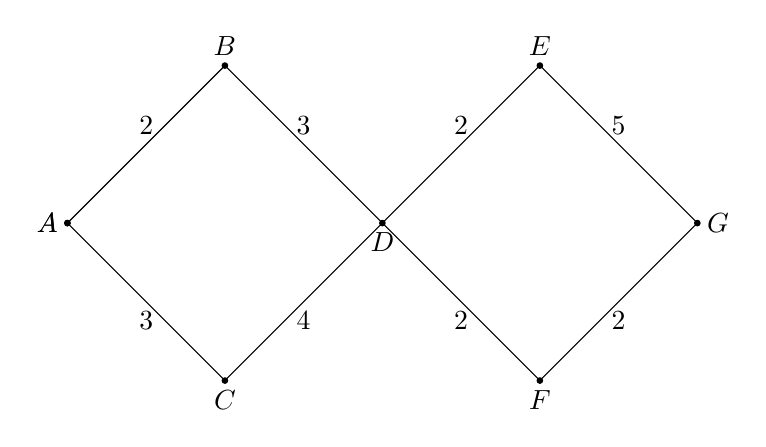
\begin{tikzpicture}[>=stealth,scale=1, line join = round, line cap = round]
	\coordinate (A) at (-3,0);
	\coordinate (B) at (-1,2);
	\coordinate (C) at (-1,-2);
	\coordinate (D) at (1,0);
	\coordinate (E) at (3,2);
	\coordinate (F) at (3,-2);
	\coordinate (G) at (5,0);
	\draw[fill=black] (A) circle (1pt) node[left] {$A$};
	\draw[fill=black] (B) circle (1pt) node[above] {$B$};
	\draw[fill=black] (C) circle (1pt) node[below] {$C$};
	\draw[fill=black] (D) circle (1pt) node[below] {$D$};
	\draw[fill=black] (A) circle (1pt) node[left] {$A$};
	\draw[fill=black] (E) circle (1pt) node[above] {$E$};
	\draw[fill=black] (F) circle (1pt) node[below] {$F$};
	\draw[fill=black] (G) circle (1pt) node[right] {$G$};
	\draw (-2,1) node [above] {$2$};
	\draw (-2,-1) node [below] {$3$};
	\draw (0,1) node [above] {$3$};
	\draw (0,-1) node [below] {$4$};
	\draw (2,1) node [above] {$2$};
	\draw (2,-1) node [below] {$2$};
	\draw (4,1) node [above] {$5$};
	\draw (4,-1) node [below] {$2$};
	
	\draw (A)-- (B)--(D)--(E)-- (G);
	\draw  (A)-- (C)-- (D)--(F)-- (G);
	
\end{tikzpicture}}
	\loigiai{
		\textbf{Cách 1.} \\
		Có $4$ lộ trình đi từ $A$ đến $G$ như sau:
		\begin{itemize}
			\item Trường hợp 1: Đi theo lộ trình $A-B-D-E-G$.
			\begin{itemize}
				\item Số cách đi từ $A$ đến $B$ là $2$ cách.
				\item Số cách đi từ $B$ đến $D$ là $3$ cách.
				\item Số cách đi từ $D$ đến $E$ là $2$ cách.
				\item Số cách đi từ $E$ đến $G$ là $5$ cách.
			\end{itemize}
			Theo quy tắc nhân, trường hợp $1$ có $2 \cdot 3 \cdot 2 \cdot 5 =60$ cách đi.
			\item Trường hợp 2: Đi theo lộ trình $A-B-D-F-G$.\\
			Tương tự như trên trường hợp $2$ có $2 \cdot 3 \cdot 2 \cdot2 =24$ cách đi.
			\item Trường hợp 3: Đi theo lộ trình $A-C-D-F-G$.\\
			Tương tự như trên trường hợp 3 có $3 \cdot 4 \cdot 2 \cdot 2=48$ cách đi.
			\item Trường hợp 4: Đi theo lộ trình $A-C-D-E-G$. \\
			Tương tự như trên trường hợp 4 có $3 \cdot 4 \cdot 2 \cdot 5=120$ cách đi.
		\end{itemize}
		Theo quy tắc cộng, số cách đi từ tỉnh $A$ đến tỉnh $G$ là $60+24+48+120=252$ cách.\\
		\textbf{Cách 2.} \\
		Đi từ $A$ đến $G$ được thực hiện bởi hai công đoạn liên tiếp như sau:
		\begin{itemize}
			\item Công đoạn 1: Đi từ $A$ đến $D$.\\
			Có 2 lộ trình đi từ $A$ đến $D$ như sau:
			\begin{itemize}
				\item Trường hợp 1: Đi theo lộ trình $A-B-D$ có $2 \cdot 3=6$ cách đi.
				\item Trường hợp 2: Đi theo lộ trình $A-C-D$ có $3 \cdot 4=12$ cách đi.
			\end{itemize}
			Theo quy tắc cộng, công đoạn $1$ có $6+12=18$ cách đi.
			\item Công đoạn 2: Đi từ $D$ đến $G$.\\
			Có 2 lộ trình đi từ $D$ đến $G$ như sau:
			\begin{itemize}
				\item Trường hợp 1: Đi theo lộ trình $D-E-G$ có $2 \cdot 5=10$ cách đi.
				\item Trường hợp 2: Đi theo lộ trình $D-F-G$ có $2 \cdot 2 =4$ cách đi.
			\end{itemize}
			Theo quy tắc cộng, công đoạn 2 có $10+4=14$ cách đi.
		\end{itemize}
		Theo quy tắc nhân, số cách đi từ tỉnh $A$ đến tỉnh $G$ là $18 \cdot 14=252$ cách.
	}
\end{baitap} \cham{11}


\begin{baitap}
	Có bao nhiêu số tự nhiên có 3 chữ số đôi một khác nhau. \\
	\hspace*{6cm} {\sf\fontsize{10pt}{1pt}\selectfont Đáp số: 648.}
	\loigiai{
		Gọi số cần tìm có dạng: $\overline{abc}$ ($a\ne 0$; $a;b;c$ đôi một khác nhau)\\
		$\Rightarrow$ Có $9\cdot9\cdot8 = 648$ số có ba chữ số.}
\end{baitap} \cham{7}

\begin{baitap}
	Cho các số $1$, $2$, $5$, $7$, $8$. Có bao nhiêu cách lập ra một số tự nhiên gồm $3$ chữ số khác nhau (các số lấy ra từ $5$ số trên) sao cho số tạo thành
	\begin{enumEX}[a)]{3}
		\item là một số chẵn;
		\item không có chữ số $7$;
		\item nhỏ hơn $278$.
	\end{enumEX}
\hspace*{6cm} {\sf\fontsize{10pt}{1pt}\selectfont Đáp số: a) 24; \quad b) 24; \quad c) 20.}
\loigiai{
}
\end{baitap} \cham{8}

\begin{baitap}
	Cho các chữ số 0, 2, 4, 5, 6, 8, 9. Từ các số trên
	\begin{tasks}(1)
		\task có thể lập được bao nhiêu số tự nhiên gồm 3 chữ số khác nhau.
		\task có thể lập được bao nhiêu số tự nhiên gồm 4 chữ số khác nhau, trong đó nhất thiết phải có mặt chữ số 5.
	\end{tasks}
	\hspace*{6cm} {\sf\fontsize{10pt}{1pt}\selectfont Đáp số: a) 180; \quad b) 420.}
	\loigiai{
	}
\end{baitap} \cham{8}


\begin{baitap}
	Cho tập hợp $A=\{0; 1; 2; 3; 4; 5; 6\}$. Hỏi từ tập hợp $A$ có thể lập được bao nhiêu số tự nhiên có $4$ chữ số khác nhau và đó là số chia hết cho $5$.\\
	\hspace*{6cm} {\sf\fontsize{10pt}{1pt}\selectfont Đáp số: 220. }
	\loigiai{
		Gọi số cần lập là $\overline{abcd}$ $(a, b, c, d\in A; a\neq b\neq c\neq d; a\neq 0; d\in\{0; 5\})$.\\
		$\bullet$ Trường hợp $d=0$: Chọn cho $a$ có $6$ cách; chọn cho $b$ có $5$ cách; chọn cho $c$ có $4$ cách. Suy ra số các số thỏa mãn bằng $6.5.4=120$ số.\\
		$\bullet$ Trường hợp $d=5$: Chọn cho $a$ có $5$ cách; chọn cho $b$ có $5$ cách; chọn cho $c$ có $4$ cách. Suy ra số các số thỏa mãn bằng $5.5.4=100$ số.\\
		Vậy có tất cả $120+100=220$ số thỏa mãn.
	}
\end{baitap} \cham{8}

\begin{baitap}
	Từ các số $0$, $1$, $2$, $3$, $4$, $5$, $6$, $7$ có thể lập ra được bao nhiêu số tự nhiên gồm 4 chữ số khác nhau và số tạo thành không chia hết cho $10$.\\
	\hspace*{6cm} {\sf\fontsize{10pt}{1pt}\selectfont Đáp số: 1260.}
	\loigiai{
	}
\end{baitap} \cham{8}

\begin{baitap}
	\immini{Hình bên mô tả $5$ xã trong một huyện. Hỏi có bao nhiêu cách mà em có thể dùng $4$ màu khác nhau để tô màu sao cho không có hai xã giáp nhau nào trùng màu?
	}{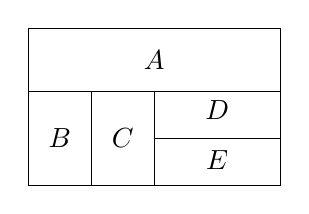
\begin{tikzpicture}[scale=0.4]
			\draw (0,3) rectangle (8,5);
			\node at (4,4) {$A$};
			\draw (0,0) rectangle (2,3);
			\node at (1,1.5) {$B$};
			\draw (2,0) rectangle (4,3);
			\node at (3,1.5) {$C$};
			\draw (4,1.5) rectangle (8,3);
			\node at (6,2.4) {$D$};
			\draw (4,0) rectangle (8,1.5);
			\node at (6,0.8) {$E$};
	\end{tikzpicture}}
	\hspace*{6cm} {\sf\fontsize{10pt}{1pt}\selectfont Đáp số: 96.}
	\loigiai{
		Theo hình vẽ
		
		Có $4$ cách tô màu xã A.
		
		Có $3$ cách tô màu xã B.
		
		Có $2$ cách tô màu xã C.
		
		Có $2$ cách tô màu xã D.
		
		Có $2$ cách tô màu xã E.
		
		Theo quy tắc nhân, có $4 \cdot 3 \cdot 2 \cdot 2 \cdot 2=96$ cách tô màu thỏa yêu cầu.
	}
\end{baitap} \cham{8}

\begin{baitap}%[1D2B1-2]
	\immini{Mã xác thực (OTP – One Time Password) do một ngân hàng gửi vào điện thoại của khách hàng cho mỗi lần giao dịch là một dãy $ 6 $ kí tự từ các chữ số từ $ 0 $ đến $ 9 $. Có thể tạo ra bao nhiêu mã xác thực khác nhau như vậy?	
	}{
		\begin{tabular}{|l|}
			\hline
			\texttt{Mã OTP xác thực giao } \\
			\texttt{dịch là $ 712892 $, hiệu}\\
			\texttt{lực trong 1 phút } $\ldots$\\ 
			\hline
	\end{tabular}}
	\hspace*{6cm} {\sf\fontsize{10pt}{1pt}\selectfont Đáp số: 1000000.}
	\loigiai{
		Có $ 10 $ cách chọn chữ số cho mỗi kí tự của mã xác nhận.\\
		Do đó theo quy tắc nhân, số mã xác nhận có thể tạo ra là $10^6=1000000$.}
\end{baitap} \cham{8}

\begin{baitap}%[1D2B1-2]
	\immini{	Một khoá tổ hợp với đĩa quay có $ 40 $ vạch số (xem hình bên). Mật mã của khoá là một dãy gồm $ 3 $ số, kí hiệu là $a-b-c$, mỗi số là một số tự nhiên từ $ 0 $ đến $ 39 $. Để mở khoá, cần quay mặt số ngược chiều kim đồng hồ cho đến khi điểm mốc gặp vạch số $a$ lần thứ ba, rồi quay mặt số theo chiều ngược lại cho đến khi điểm mốc gặp vạch số $b$ lần thứ hai, cuối cùng quay mặt số ngược chiều kim đồng hồ cho đến khi điểm mốc gặp vạch số $c$ lần đầu tiên. Nếu $a$, $b$, $c$ phải khác nhau đôi một, thì có bao nhiêu cách chọn mật mã cho khoá tổ hợp trên?	}{
		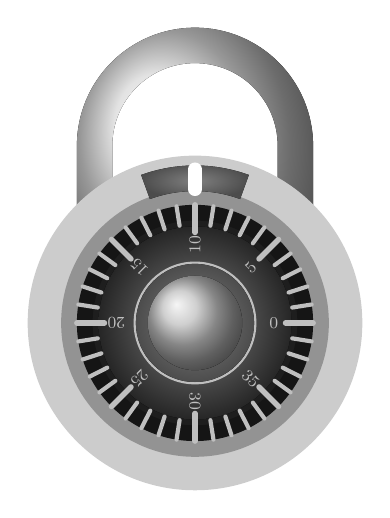
\begin{tikzpicture}[font=\footnotesize, line join=round, line cap=round, >=stealth,scale=0.5]
			\begin{scope}[transform shape]
				\tikzset{Khoa-mat-ma/.pic={
						\def\R{3}
						\def\g{9}
						\fill[ball color=gray!30](-\R,0)--++(90:1.5*\R)arc(180:0:\R)--(\R,0)--(0.7*\R,0)--++(90:1.5*\R)arc(0:180:0.7*\R)--(-0.7*\R,0)--cycle;
						\fill[gray!40](0,0)circle(\R+1.25);
						\draw[gray,line width=4mm,opacity=0.75](0,0)circle(\R);
						\fill[opacity=0.85](0,0)circle(\R);
						\fill[outer color=black!85](0,0)circle(\R-0.55);
						\fill[gray!50](0,0)circle(0.52*\R);
						\fill[outer color=black!70](0,0)circle(0.5*\R);
						\fill[ball color=gray!50](0,0)circle(0.4*\R);
						\fill[outer color=black!70](70:{\R+1})arc(70:110:{\R+1})--(110:\R+0.35)arc(110:70:{\R+0.35});
						\draw[white,line width=5pt](90:\R+0.4)--++(90:0.5);
						\foreach \i in{0,9,...,354}{
							\pgfmathsetmacro{\k}{int(mod(\i,5))}
							\pgfmathsetmacro{\m}{int(\i/9)}
							\draw[white!50!gray,line width=1.5pt](\i:\R)--++(180+\i:0.5);
							\ifnum \k=0
							\draw[white!50!gray,line width=2pt](\i:\R)--++(180+\i:0.7);
							\path(\i*\g:\R)++(180+\i*\g:1)node[scale=1.5,rotate=\i]{\color{white!50!gray}$\m$};
							\fi
				}}}
				\path(0,0)pic{Khoa-mat-ma};
			\end{scope}
	\end{tikzpicture}}
	\hspace*{6cm} {\sf\fontsize{10pt}{1pt}\selectfont Đáp số: 59280.}
	\loigiai{
		Có $ 40 $ cách chọn số $a$ từ các số từ $ 0 $ đến $ 39 $. Tiếp theo, có $ 39 $ cách chọn số $b$ từ $ 39 $ số còn lại. Cuối cùng, có $ 38 $ cách chọn số $c$ từ $ 38 $ số còn lại. Áp dụng quy tắc nhân, ta có $40\cdot 39\cdot 38 = 59280$ cách chọn mật mã cho khoá.}
\end{baitap} \cham{8}


\begin{baitap}%[1D2B1-2]
	\immini{Mã số nhân viên của một công ty có $ 4 $ kí tự, gồm một chữ cái đầu tiên (từ $ 6 $ chữ cái $ A $, $ B $, $ C $, $ D $, $ E $, $ F $) và tiếp theo là $ 3 $ chữ số (từ các chữ số $0, 1, \ldots ,9$). Công ty có thể tạo ra bao nhiêu mã số nhân viên theo cách này?	}{
		\begin{tikzpicture}
			\path
			(0,0) coordinate (A)
			($ (A)+(6,0) $) coordinate (B)
			($ (A)+(0,2.5) $) coordinate (D)
			($ (A)+(0,3.5) $) coordinate (M)
			($ (B) +(0,2.5) $) coordinate (C)
			($ (B) +(0,3.5) $) coordinate (N)
			($ (A)!0.8 !(D)$) coordinate (E)
			($ (B)!0.8 !(C)$) coordinate (F)
			($ (E)!0.45!(F) $) coordinate (E1)		
			($ (E)!0.55!(F) $) coordinate (F1)
			($ (M)!0.55!(N) $) coordinate (M1)
			($ (M)!0.45!(N) $) coordinate (N1)
			($ (E)!0.5!(F) $) coordinate (F11)
			($ (A)!0.5!(B) $) coordinate (F12)
			;
			\draw 
			(A)--(B)--(C)--(D)--cycle  (E1)--(F1)--(M1)--(N1)--cycle;
			\draw (0.2,0.8) --(1.5,0.8)--(1.5,1.8)--(.2,1.8)--cycle (1.7/2,2.6/2) node{Ảnh};
			\draw (1.1,0.4) node{\fbox{\tiny {Mã số:ABCD123}}} (F11)--(F12);
			\draw (4.5,2)node[below]{\tiny THẺ NHÂN VIÊN};
	\end{tikzpicture}}
	\hspace*{6cm} {\sf\fontsize{10pt}{1pt}\selectfont Đáp số: 6000.}
	\loigiai{
		Có $ 6 $ cách chọn chữ cái cho kí tự đầu tiên.\\
		Với $ 3 $ kí tự tiếp theo, mỗi kí tự có $ 10 $ cách chọn từ 10 chữ số $0,1,2,\ldots,9$.\\
		Theo quy tắc nhân, công ty có thể tạo ra $6 \cdot 10 \cdot 10 \cdot 10=6000$ mã số nhân viên.}
\end{baitap} \cham{8}

\begin{baitap}%[1D2B1-1]
	\immini{Tung đồng thời hai con xúc xắc khác nhau và ghi lại số chấm xuất hiện trên mỗi con xúc xắc. Có bao nhiêu kết quả có thể xảy ra mà tổng số chấm xuất hiện trên hai mặt là bội của $ 5 $?	}{
		\begin{tikzpicture}	
			\tikzset{motcham/.pic={
					\begin{scope}[rounded corners=2mm]
						\def\a{2}
						\path(0,0)coordinate(A)++(-30:0.85*\a)coordinate(B)(1.5*\a,0)coordinate(C)($(A)+(C)-(B)$)coordinate(D);
						\path[shift={(0,\a)}](0,0)coordinate(A')++(-30:0.85*\a)coordinate(B')(1.5*\a,0)coordinate(C')($(A')+(C')-(B')$)coordinate(D');
						\fill[gray,draw=gray](A)--(A')--(D')--(C')--(C)--(B)--cycle;
						\draw[fill=gray!30,draw=gray](B)--(C)--(C')--(B')--cycle (A')--(B')--(C')--(D')--cycle (A)--(A')--(B')--(B)--cycle;
						\fill[ball color=red,yscale=0.5,draw=red!30]($(A')!0.5!(C')$)circle(0.25*\a)($(A')!0.5!(C')$)circle(0.25*\a);
						\path($(A')!0.5!(B')$)coordinate(M')($(A)!0.5!(B)$)coordinate(M);
						\fill[ball color=red,yslant=-0.3,,draw=red!30]($(M)!1/3!(M')$)circle(0.125*\a)($(M)!2/3!(M')$)circle(0.125*\a);
						\path($(B')!1/3!(C')$)coordinate(N')($(B) !1/3!(C)$)coordinate(N)($(B')!2/3!(C')$)coordinate(P')($(B)!2/3!(C)$)coordinate(P);
						\fill[ball color=red,yslant=0.3,draw=red!30]($(N)!1/3!(N')$)circle(0.1*\a)($(N)!2/3!(N')$)circle(0.1*\a)($(P)!1/3!(P')$)circle(0.1*\a)($(P)!2/3!(P')$)circle(0.1*\a);
					\end{scope}
			}}
			\path(0,0)pic{motcham};
			\path (3.5,0) pic{motcham};
	\end{tikzpicture}}
	\hspace*{6cm} {\sf\fontsize{10pt}{1pt}\selectfont Đáp số:7.}
	\loigiai{
		Ta viết $(a,b)$ để kí hiệu kết quả số chấm xuất hiện trên hai con xúc xắc lần lượt là $a$ và $b$. \\
		Ta có $2 \leq a+b \leq 12$ nên $a+b$ là bội của $ 5 $ khi $a+b=5$ hoặc $a+b=10$.
		\begin{itemize}
			\item Trường hợp $a+b=5$ gồm các kết quả: $(1,4),(2,3),(3,2),(4,1)$.\\ Trường hợp này có $ 4 $ kết quả.
			\item Trường hợp $a+b=10$ bao gồm các kết quả: $(4,6),(5,5),(6,4)$.\\ Trường hợp này có $ 3 $ kết quả.
		\end{itemize} 
		Vậy có $4+3=7$ kết quả có thể xảy ra mà tổng số chấm xuất hiện trên hai con xúc xắc là bội của $ 5 $.}
\end{baitap} \cham{8}

